\documentclass{article}
\usepackage[utf8]{inputenc}
\usepackage[T1]{fontenc}
\usepackage[russian]{babel}
\usepackage{tikz}
\usepackage{graphicx}
\usepackage{titlesec}
\usepackage{amsfonts}
\usepackage{amsmath}
\usepackage[left=2cm,right=2cm,
    top=2cm,bottom=2cm,bindingoffset=0cm]{geometry}
\renewcommand{\thesection}{\arabic{section}}
\titleformat{\section}{\large\bfseries}{\thesection}{1em}{}
\title{Интегрирование}
\author{Каренин Константин Витальевич}
\date{02.04.2024}
\begin{document}

\begin{titlepage}
    \centering
    \vspace*{0.5 cm}
    
    \textsc{\LARGE \textbf{Специальные разделы высшей математики}}
    \vspace{1.5cm}
    
    \rule{\linewidth}{0.2 mm} \\[0.4 cm]
    { \huge \bfseries Линейная алгебра}
    \rule{\linewidth}{0.2 mm} \\[1.5 cm]
    
    \Large Выполнили: \\
    Каренин Константин \\
    Темиров Тимур \\
    Гонин Сергей \\
    Малышева Алиса \\
    
    \vspace{0.5cm}
    
    Группа: М3104
    
    \vspace{0.5cm}
    
    Преподаватель: Сарычев Павел
    
    \vspace{0.5cm}
    
    Университет ИТМО
    
    \vfill

    
\includegraphics[height=70px]{logo.jpg}
    
    2.04.2024
    
\end{titlepage}

\setcounter{page}{2}

% task 1
\newpage
    \section{Евклидовы пространства функций}
    \subsection{Дано пространство многочленов с вещественными коэффициентами, степени не выше третьей,
определенных на отрезке $[-1; 1]$.}
    \subsubsection{Проверьте, что система векторов $B = \{1, t, t^2, t^3\}$ является базисом этого пространства.
Ортогонализируйте систему (построенный ортогональный базис обозначьте $B_H$)}
    Проверим, что данная система линейно независима:
    $P(t) =  C_1 + C_2t + C_3t^2 + C_4t^3 = 0 \; \forall t \in \mathbb{R}$\\
    \begin{equation*}
        \begin{cases}
            P(0) = 0 \Rightarrow C_1 = 0 \\
            P(1) = C_1 + C_2 + C_3 + C_4 = 0 \\
            P(-1) = C_1 - C_2 + C_3 - C_4 = 0 \\
            P(2) = C_1 + 2C_2 + 4C_3 + 8C_4 = 0 \\
        \end{cases}
    \end{equation*}
    \begin{equation*}
        \begin{cases}
            C_1 = 0 \\
            C_1 + C_2 + C_3 + C_4 = 0 \\
            - C_2 + C_3 - C_4 = 0 \\
            2C_3 + 6C_4 = 0 \\
        \end{cases}
        \begin{cases}
            C_1 = 0 \\
            C_3 = 0 \\
            C_2 + C_3 + C_4 = 0 \\
            2C_3 + 6C_4 = 0 \\
        \end{cases}
        \begin{cases}
            C_1 = 0 \\
            C_3 = 0 \\
            C_4 = 0 \\
            C_2 = 0 \\
        \end{cases}
        \Rightarrow
        B - \text{линейно независимый}
        \Rightarrow
        B - \text{базис}
    \end{equation*}
    Ортогонализируем базис методом Грамма-Шмидта\\
    Пусть $f_1 = 1$\\
    $f_2 = t + \alpha f_1$\\
    $\alpha = - \frac{(t, 1)}{2} = - \frac{\int_{-1}^1 t dt}{2} = 0 \Rightarrow f_2 = t$\\
    $f_3 = t^2 + \beta t + \alpha$\\
    $\beta = - \frac{(t^2, t)}{(t, t)} = - \frac{\int_{-1}^0 t^3 dt}{\int_{-1}^1 t^2 dt} = 0$\\
    $\alpha = - \frac{(t^2, 1)}{(1, 1)} = -\frac{1}{2} \int_{-1}^1 t^2 dt = - \frac{1}{3}$\\
    $\Rightarrow f_3 = t^2 - \frac{1}{3}$\\
    $f_4 = t^3 + \alpha(t^2 - \frac{1}{3}) + \beta t + \gamma$\\
    $\alpha = - \frac{(t^3, t^2 - \frac{1}{3})}{(t^2 - \frac{1}{3}, t^2 - \frac{1}{3})} = - \frac{\int_{-1}^1 (t^5 - \frac{1}{3}t^3) dt}{\int_{-1}^1 (t^4 - \frac{2}{3}t^2 + \frac{1}{9}) dt} = 0$\\
    $\beta = - \frac{(t^3, t)}{(t, t)} = \frac{\int_{-1}^1 t^4 dt}{\int_{-1}^1 t^2 dt} = - \frac{3}{5}$\\
    $r = - \frac{(t^3, 1)}{(1, 1)} = - \frac{\int_{-1}^1 t^3 dt}{2} = 0$\\
    $f_4 = t^3 - \frac{3}{5} t$\\
    $B_H = \{1, t, t^2 - \frac{1}{3}, t^3 - \frac{3}{5}t\}$ - ортогональный базис
    
    \subsubsection{Выпишите первые четыре (при $n = 0, 1, 2, 3$ ) многочлена Лежандра: $L_n (t) = \frac{1}{2^n n!} \frac{d^n}{dt^n}((t^2-1)n)$, 
    где $\frac{d^n}{dt^n} (y(t))$ - производная $n$-ого порядка функции $y(t)$}
    $L_n (t) = \frac{1}{2^n n!} \frac{d^n}{dt^n} ((t^2-1)^n)$\\
    $L_0 (t) = 1$\\
    $L_1 (t) = \frac{1}{2} 2t = t$\\
    $L_2 (t) = \frac{1}{8} \frac{d^2}{dt^2}((t^2-1)^2) = \frac{3t^2}{2} - \frac{1}{2}$\\
    $L_3 (t) = \frac{1}{48} \frac{d^3}{dt^3}((t^2-1)^3) = \frac{5t^3}{2} - \frac{3}{2}t$
    
    \subsubsection{Найдите координаты полученных многочленов $L_n(t)$ в базисе $B_H$. Сделайте вывод об ортогональности системы векторов $L_n(t)$.}
    $L_0 (t) = (1, 0, 0, 0)_{B_H}$\\
    $L_0 (t) = (0, 1, 0, 0)_{B_H}$\\
    $L_0 (t) = (0, 0, \frac{3}{2}, 0)_{B_H}$\\
    $L_0 (t) = (0, 0, 0, \frac{5}{2})_{B_H}$\\
    Система векторов ортогональна, поскольку скалярные произведения векторов равны 0.
    
    \subsubsection{Разложите данный многочлен $P_3(t) =  t^3 - 2t^2 + t + 1$ по системе векторов $L_n(t)$}
    $P_3 (t) = t^3 -2t^2 + t + 1$\\
    $P_3 (t) = (\frac{1}{3}, 1\frac{3}{5}, -2, 1)_{B_H} = \frac{1}{3}(1, 0, 0, 0)_{B_H} + 1\frac{3}{5}(0, 1, 0, 0)_{B_H} - \frac{4}{3}(0, 0, \frac{3}{2}, 0)_{B_H} + \frac{2}{5}(0, 0, 0, \frac{5}{2})_{B_H} =  \frac{1}{3}L_0(t) + 1\frac{3}{5}L_1(t) - \frac{4}{3}L_2(t) + \frac{2}{5}L_3(t)$\\
    $P_3(t) = (\frac{1}{3}, 1\frac{3}{5}, -\frac{4}{3}, \frac{2}{5})_{L(t)}$
    
    
    \subsection{Дано пространство $R$ функций, непрерывных на отрезке $[-\pi ; \pi]$ со скалярным произведением $(f, g) = \int_{-\pi}^\pi f(t)g(t) dt$ и длиной вектора $||f|| = \sqrt{(f, f)}$.\\
    Тригонометрические многочлены $P_n(t)= \frac{a_0}{2} + a_1 \cos t + b_1 \sin t + ... + a_n \cos nt + b_n \sin nt$, где $a_k, b_k$ - вещественные коэффициенты, образуют подпространство $P$ пространства $R$.\\
    Требуется найти многочлен $P_n(t)$ в пространстве $P$, минимально отличающийся от функции $f(t)$ - вектора пространства $R$.}
    \subsubsection{Проверьте, что система функций $\{1, \cos t, \sin t, ... \cos nt, \sin nt\}$ является ортогональным базисом подпространства $P$. Нормируйте систему.}
    Для того, чтобы проверить, что система функций ортогональна, нам необходимо проверить скалярные произведения элементов системы: они должны быть равны 0, чтобы они были ортогональными.\\
    Рассмотрим общие случаи для $\cos mx$ и $\sin kx$ из этих функций можно получить любой элемент системы.\\
    Рассмотрим скалярные произведения обобщённых элементов:\\
    $\int_{-\pi}^\pi \cos mx \sin kx \; dx = \frac{1}{2} \int_{-\pi}^\pi (\sin(kx - mx) + \sin(kx + mx)) \; dx = \int_{0}^\pi \sin(kx-mx) \; dx + \int_{0}^\pi \sin(kx+mx) \; dx = 0$, \\
    т.к. $\int_{0}^\pi \sin mx \; dx = 2(\frac{\cos m \pi}{m} - \frac{\cos 0}{m}) = 0$\\
    $\int_{-\pi}^\pi \cos mx \cos kx \; dx = \int_{0}^\pi \cos(mx-kx) \; dx + \int_{0}^\pi \cos (mx-kx) = 0$, \\
    т.к. $\int_{-\pi}^\pi \cos mx \; dx = 2(\frac{\sin m \pi}{m} - \frac{\sin 0}{m}) = 0$\\
    $\int_{-\pi}^\pi \sin mx \sin kx \; dx = \int_{0}^\pi \cos(mx-kx) \; dx - \int_{0}^\pi \cos (mx+kx) \; dx = 0$\\
    Скалярные произведения обобщённых элементов равны 0 $\Rightarrow$ скалярные произведения системы равны 0 $\Rightarrow$ элементы системы ортогональны\\
    Чтобы нормировать систему, надо вычислить норму элементов, чтобы эти элементы поделить на собственную "длину", получив "единичные" элементы. \\
    Вычислим нормы для обобщённых элементов, чтобы получить нормы для элементов системы: \\
    $|| \cos mx || = \sqrt{\int_{-\pi}^\pi \cos^2 mx \; dx} = \sqrt{2\int_{0}^\pi \cos^2 mx \; dx }= \sqrt{\int_{0}^\pi 2\cos^2 mx \; dx }= \sqrt{\int_{0}^\pi (\cos 2mx + 1)\; dx} = \sqrt{\int_{0}^\pi dx} = \sqrt{\pi}$\\
    $|| \sin mx || = \sqrt{\int_{-\pi}^\pi \sin^2 mx \; dx} = \sqrt{\int_{-\pi}^\pi \frac{1 - \cos 2mx}{2} \; dx} = \sqrt{\pi}$\\
    $||1|| = \sqrt{\int_{-\pi}^\pi \; dx} = \sqrt{2 \pi}$ \\
    Теперь мы можем получить нормированную систему:\\
    $N = \{\frac{1}{\sqrt{2\pi}}, \frac{\sin x}{\sqrt{\pi}}, \frac{\cos x}{\sqrt{\pi}}, ... , \frac{\sin mx}{\sqrt{\pi}}, \frac{\cos mx}{\sqrt{\pi}}\} -$ ортонормированная система
    
    \subsubsection{Найдите проекции вектора $f(t) = 2t$ на векторы полученного ортонормированного базиса.}
    Проекция $f(t)$ на $g(t)$ определяется:
    $Proj_{g(t)} f(t) = \frac{(f(t), g(t)}{||g(t)||} g(t)$\\
    $Proj_{1} 2x = \frac{\int_{-\pi}^\pi 2x dx}{\sqrt{\int_{-\pi}^\pi 1 dx}} = 0$\\
    $Proj_{\cos mx} 2x = g(x) \frac{\int_{-\pi}^\pi 2x \cos mx dx}{\sqrt{\pi}} = 0$\\
    $Proj_{\sin mx} 2x = \frac{2 \int_{-\pi}^\pi x \sin x dx}{\sqrt{\pi}} \sin x = - \frac{2 \pi \cos \pi m \sin mx}{m}$\\
    
    
    \subsubsection{Запишите минимально отстоящий многочлен $P_n(t)$ с найденными коэффициентами (тригонометрический многочлен Фурье для данной функции).}
    $f(x) \sim \frac{a_0}{2} + \sum_{n=1}^{\infty}(a_u \cos mx + bm sin mx)$ - тригонометрический многочлен Фурье\\
    $a_0 = \frac{1}{\pi} \int_{-\pi}^\pi 2x \; dx = 0$\\
    $a_n = \frac{1}{\pi} \int_{-\pi}^\pi 2x \cos nx \; dx = 0$\\
    $b_n = \frac{1}{\pi} \int_{-\pi}^\pi 2x \sin nx \; dx = -\frac{4 \cos \pi n}{n}$\\
    По-сути $\cos \pi n$ мы можем представить, как $(-1)^n$, т.к. функции $\cos n \pi$ и $(-1)^n$ периодичный, причём для $n$ одной и той же чётности (в частности, для одних и тех же $n$) результат будет одинаковым\\
    $f(x) \sim \sum_{n=1}^{\infty}(- \frac{4(-1)^n}{n} \sin t)$
     
    \subsubsection{Изобразите графики функции $f(t)$ и многочлена Фурье различных порядков $n$}
    \begin{equation*}
        n = 4 \; \; \; \; \; \; \; \; \; \; \; \; \; \; \; \; \; \;
        \; \; \; \; \; \; \; \; \;
        n = 100 \; \; \; \; \; \; \; \; \; \; \; \; \; \; \; \; \; \;
        \; \; \; \; \; \; \; \; \;
        n = 1000 \; \; \; \; \; \; \; \; \; \; \; \; \; \; \; \; \; \;
        \; \; \; \; \; \; \; \; \;
        n = +\infty
    \end{equation*}
    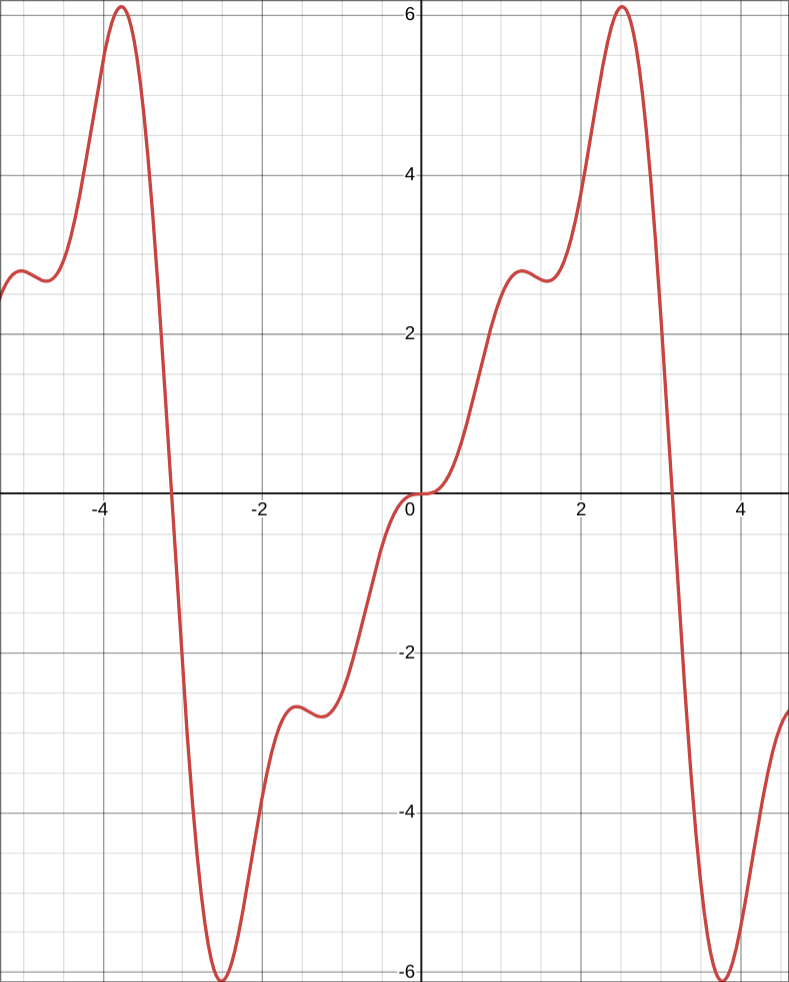
\includegraphics[height=200px]{rgr1.1.png}
    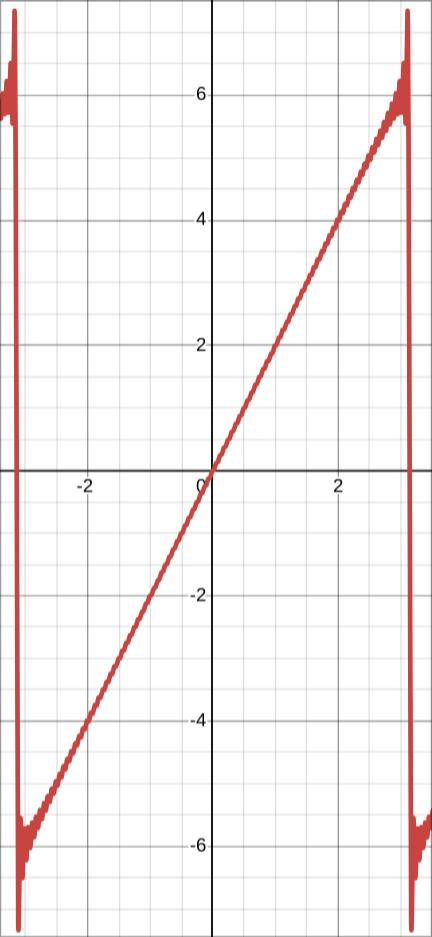
\includegraphics[height=200px]{rgr1.2.png}
    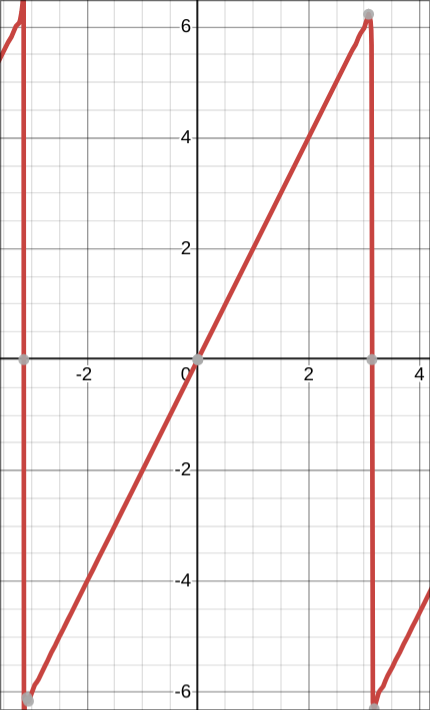
\includegraphics[height=200px]{rgr1.3.png}
    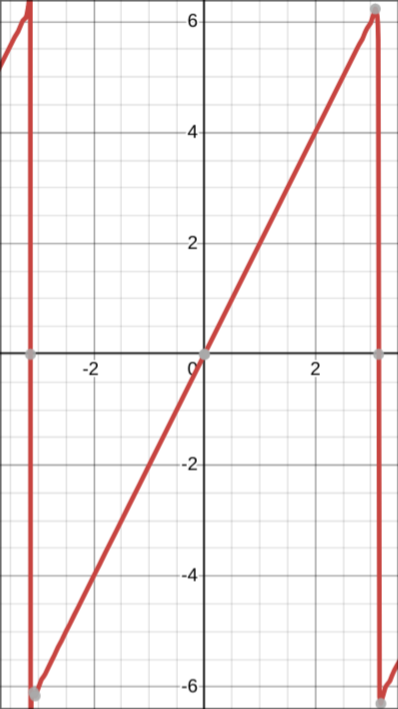
\includegraphics[height=200px]{rgr1.4.png}
    
    \subsubsection{Сделайте вывод о поведении многочлена при росте его порядка.}
    При росте порядка многочлена уменьшается "отстояние" \;графика многочлена Фурье от самой функции.
    
    
    
    

    
% task 2
\newpage
    \section{Приведение уравнения поверхности 2-го порядка к каноническому виду}
    Дано уравнение поверхности 2-го порядка: $2x^2 - 6xy + 2y^2 + z^2 - 25 = 0$
    \subsection{Составьте матрицу квадратичной формы и диагонализируйте ее. Запишите канонический базис
    квадратичной формы.}
    $F(x, y, z) = 2x^2 -6xy + 2y^2 + z^2$ \\
    Составим матрицу квадратичной формы: \\
    \begin{equation*}
    A = 
        \begin{pmatrix}
            2& -3& 0\\
            -3& 2& 0\\
            0& 0& 1\\
        \end{pmatrix}
    \end{equation*}
    Из определения собственного вектора $v$ соответствующего собственному значению $\lambda$: $A v=\lambda v$ \\
    Тогда: $A v-\lambda v=(A-\lambda E) v=0$\\
    Уравнение имеет ненулевое решение тогда и только тогда, когда
    det$(A-\lambda E) = 0$
    \[
    det(A-\lambda E) =
    \begin{vmatrix}
    2-\lambda & -3 & 0 \\
    -3 & 2-\lambda & 0 \\
    0 & 0 & 1-\lambda
    \end{vmatrix}
     = -\lambda^3 +5 \lambda^2 + \lambda -5 
    \]
    $- (\lambda-1) \cdot (\lambda+1) \cdot (\lambda-5) = 0$
    Для каждого λ найдем его собственные вектора: \\
    1. $\lambda_1 = -1$
    \begin{equation*}
    A -\lambda_1 E = 
        \begin{pmatrix}
            3& -3& 0 \\
            -3& 3& 0 \\
            0& 0& 2 \\
        \end{pmatrix}
    \end{equation*}
    \begin{equation*}
        \begin{pmatrix}
            3& -3& 0 \text{ |  0}\\
            -3& 3& 0 \text{ |  0}\\
            0& 0& 2  \text{ |  0}\\
        \end{pmatrix}
         =
         \begin{pmatrix}
            1& -1& 0 \text{ |  0}\\
            -3& 3& 0 \text{ |  0}\\
            0& 0& 2 \text{ |  0}\\
        \end{pmatrix}
        =
        \begin{pmatrix}
            1& -1& 0 \text{ |  0}\\
            0& 0& 0 \text{ |  0}\\
            0& 0& 2 \text{ |  0}\\
        \end{pmatrix}
        =
        \begin{pmatrix}
            1& -1& 0 \text{ |  0}\\
            0& 0& 0 \text{ |  0}\\
            0& 0& 2 \text{ |  0}\\
        \end{pmatrix}
        =
        \begin{pmatrix}
            1& -1& 0 \text{ |  0}\\
            0& 0& 1 \text{ |  0}\\
            0& 0& 0 \text{ |  0}\\
        \end{pmatrix}
    \end{equation*}
    \begin{equation*}
        \begin{cases}
            x_1 - x_2 = 0 \\
            x_3= 0 \\
        \end{cases}
    \end{equation*}
    \begin{equation*}
   \widetilde{v_1} = 
        \begin{pmatrix}
            1\\
            1 \\
            0  \\
        \end{pmatrix}
    \end{equation*}
    2. $\lambda_2 = 1$
    \begin{equation*}
    A -\lambda_2 E = 
        \begin{pmatrix}
            1& -3& 0 \\
            -3& 1& 0 \\
            0& 0& 0  \\
        \end{pmatrix}
    \end{equation*}
    \begin{equation*}
        \begin{pmatrix}
            1& -3& 0 \text{ |  0}\\
            -3& 1& 0 \text{ |  0}\\
            0& 0& 0  \text{ |  0}\\
        \end{pmatrix}
         =
         \begin{pmatrix}
            1& -3& 0 \text{ |  0}\\
            0& -8& 0 \text{ |  0}\\
            0& 0& 0 \text{ |  0}\\
        \end{pmatrix}
        =
        \begin{pmatrix}
            1& -3& 0 \text{ |  0}\\
            0& 1& 0 \text{ |  0}\\
            0& 0& 0 \text{ |  0}\\
        \end{pmatrix}
        =
        \begin{pmatrix}
            1& 0& 0 \text{ |  0}\\
            0& 1& 0 \text{ |  0}\\
            0& 0& 0 \text{ |  0}\\
        \end{pmatrix}
    \end{equation*}
       \begin{equation*}
        \begin{cases}
            x_1= 0 \\
            x_2= 0 \\
            x_3 = x_3 \\
        \end{cases}
    \end{equation*}
    \begin{equation*}
    \widetilde{v_2} = 
        \begin{pmatrix}
            0\\
            0 \\
            1  \\
        \end{pmatrix}
    \end{equation*}
    3. $\lambda_3 = 5$
    \begin{equation*}
    A -\lambda_2 E = 
        \begin{pmatrix}
            -3& -3& 0 \\
            -3& -3& 0 \\
            0& 0& -4  \\
        \end{pmatrix}
        \end{equation*}
        \begin{equation*}
        \begin{pmatrix}
            -3& -3& 0 \text{ |  0}\\
            -3& -3& 0 \text{ |  0}\\
            0& 0& -4  \text{ |  0}\\
        \end{pmatrix}
         =
         \begin{pmatrix}
            1& 1& 0 \text{ |  0}\\
            -3& -3& 0 \text{ |  0}\\
            0& 0& -4 \text{ |  0}\\
        \end{pmatrix}
        =
        \begin{pmatrix}
            1& 1& 0 \text{ |  0}\\
            0& 0& 0 \text{ |  0}\\
            0& 0& -4 \text{ |  0}\\
        \end{pmatrix}
        =
        \begin{pmatrix}
            1& 1& 0 \text{ |  0}\\
            0& 0& 1 \text{ |  0}\\
            0& 0& 0 \text{ |  0}\\
        \end{pmatrix}
    \end{equation*}
       \begin{equation*}
        \begin{cases}
            x_1 + x_2 = 0 \\
            x_3 = x_3 \\
        \end{cases}
    \end{equation*}
    \begin{equation*}
    \widetilde{v_3} = 
        \begin{pmatrix}
            -1\\
            1 \\
            0  \\
        \end{pmatrix}
    \end{equation*}
    Собственные числа и векторы:
    \begin{equation*}
        \lambda_1 = -1 \; \; \; \; \; \; 
        \widetilde{v_1}=
        \begin{pmatrix}
            1\\
            1\\
            0\\
        \end{pmatrix}
    \end{equation*}
    \begin{equation*}
        \lambda_2 = 1 \; \; \; \; \; \; 
        \widetilde{v_2}=
        \begin{pmatrix}
            0\\
            0\\
            1\\
        \end{pmatrix}
    \end{equation*}
    \begin{equation*}
        \lambda_3 = 5 \; \; \; \; \; \; 
        \widetilde{v_3}=
        \begin{pmatrix}
            -1\\
            1\\
            0\\
        \end{pmatrix}
    \end{equation*}
    \begin{equation*}
        \begin{cases}
            v_1= \frac{\widetilde{v_1}}{\text{||} \widetilde{v_1} \text{||}} =
            \begin{pmatrix}
                \frac{1}{\sqrt{2}}\\
                \frac{1}{\sqrt{2}}\\
                0\\
            \end{pmatrix}\\
            v_2= \frac{\widetilde{v_2}}{\text{||} \widetilde{v_2} \text{||}} =
            \begin{pmatrix}
                0\\
                0\\
                1\\
            \end{pmatrix}\\
            v_3= \frac{\widetilde{v_3}}{\text{||} \widetilde{v_3} \text{||}} =
            \begin{pmatrix}
                -\frac{1}{\sqrt{2}}\\
                \frac{1}{\sqrt{2}}\\
                0\\
            \end{pmatrix}\\
        \end{cases} - \text{ортонормированный базис}
    \end{equation*}
    $\{e_1, e_2, e_3\} = \{i, j, k\}$\\
    $\forall u \in \mathbb{R} \; \; \; \;$
    $u_e = T_{e \to v} u_v$ \\
    Теперь составим из собственных векторов ортогональную матрицу перехода:
    \begin{equation*}
        \begin{pmatrix}
            x\\
            y\\
            z\\
        \end{pmatrix}
        =
        \begin{pmatrix}
            \frac{1}{\sqrt{2}}& 0& - \frac{1}{\sqrt{2}}\\
            \frac{1}{\sqrt{2}}& 0& \frac{1}{\sqrt{2}}\\
            0& 1& 0\\
        \end{pmatrix}
        \begin{pmatrix}
            x'\\
            y'\\
            z'\\
        \end{pmatrix}
    \end{equation*}
    \begin{equation*}
        \begin{cases}
            x = \frac{1}{\sqrt{2}}x' - \frac{1}{\sqrt{2}}z'\\
            y = \frac{1}{\sqrt{2}}x' + \frac{1}{\sqrt{2}}z'\\
            z = y'\\
        \end{cases}
    \end{equation*}
    $2x^2 - 6xy +2 y^2 + z^2 - 25 =0$ \\
    $ x'^2 - 2x'z' + z'^2 - 3x'^2 + 3z'^2 + x'^2 + 2x'z'+z'^2 + y'^2 - 25 = 0$\\
    $-x'^2 + y'^2 + 5z'^12 = 25$ \\
    $\frac{y'^2}{25} + \frac{z^2}{5} - \frac{x'^2}{25} = 1$ \\

    
    \begin{equation*}
        \begin{pmatrix}
            -1& 0& 0\\
            0& 1& 0\\
            0& 0& 5\\
        \end{pmatrix}
        - \text{матрица квадратичной формы}
    \end{equation*}
    \begin{equation*}
        \begin{cases}
            \sqrt{2}x=x'-z'\\
            \sqrt{2}y=x'+z'\\
            z=y'\\
        \end{cases}
        \begin{cases}
            x'=\sqrt{2}x+z'\\
            \sqrt{2}y=\sqrt{2}x+2z'\\
            z=y'\\
        \end{cases}
        \begin{cases}
            2z'=\sqrt{2}y-\sqrt{2}x\\
            x'=\sqrt{2}x+z'\\
            z = y'\\
        \end{cases}
        \begin{cases}
            z'=\frac{\sqrt{2}}{2}y-\frac{\sqrt{2}}{2}x\\
            x'=\frac{\sqrt{2}}{2}x+\frac{\sqrt{2}}{2}y\\
            y'=z\\
        \end{cases}
    \end{equation*}
    $\{x', y', z'\}$ - канонический базис\\
    
    \subsection{Классифицируйте поверхность по ее каноническому уравнению.}
    Канонический вид данного выражения:\\
    $\frac{y'^2}{25} + \frac{z^2}{5} - \frac{x'^2}{25} = 1$ - однополосный гиперболоид \\
    \subsection{Определите, каким преобразованием пространства поверхность была приведена к главным
осям.}
    Если мы посмотри на матрицу преобразования:
     \begin{pmatrix}
            \frac{1}{\sqrt{2}}& 0& - \frac{1}{\sqrt{2}}\\
            \frac{1}{\sqrt{2}}& 0& \frac{1}{\sqrt{2}}\\
            0& 1& 0\\
        \end{pmatrix}
    То можем заметить, что у нас происходили измения координат, по всем осям, кроме $y$ и данная матрица, является матрицей поворота, причём поворот выполняется относительно оси $Oz$ на угол $\frac{-\pi}{4}$ и относительно оси $Ox$ на $\frac{\pi}{2}$ \\
    Значит мы можем сказать, что преобразованием является поворот.

    \subsection{Изобразите график уравнения в исходной системе координат. Укажите на графике оси исходной и приведённой систем координат.}
    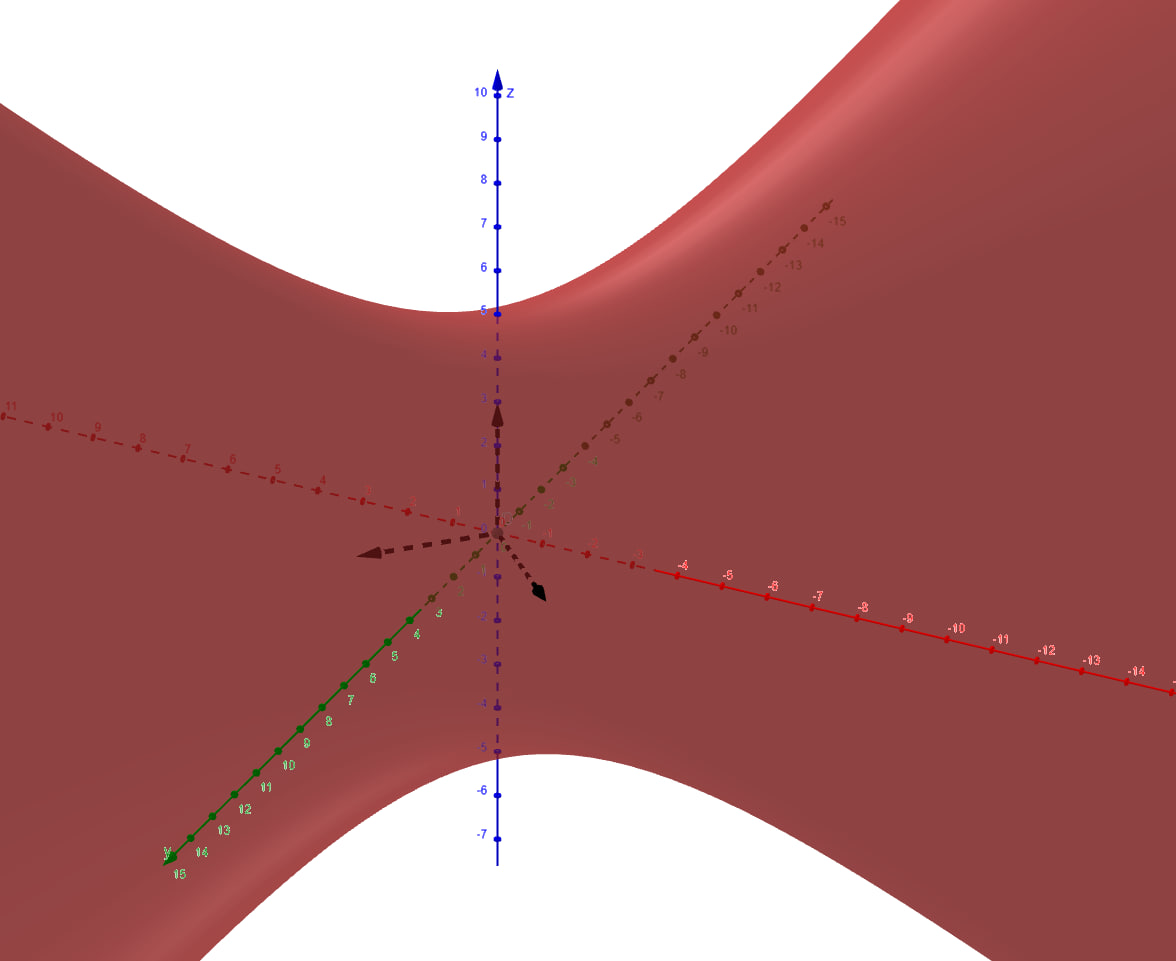
\includegraphics[height=200px]{rgr2.1.jpg}
    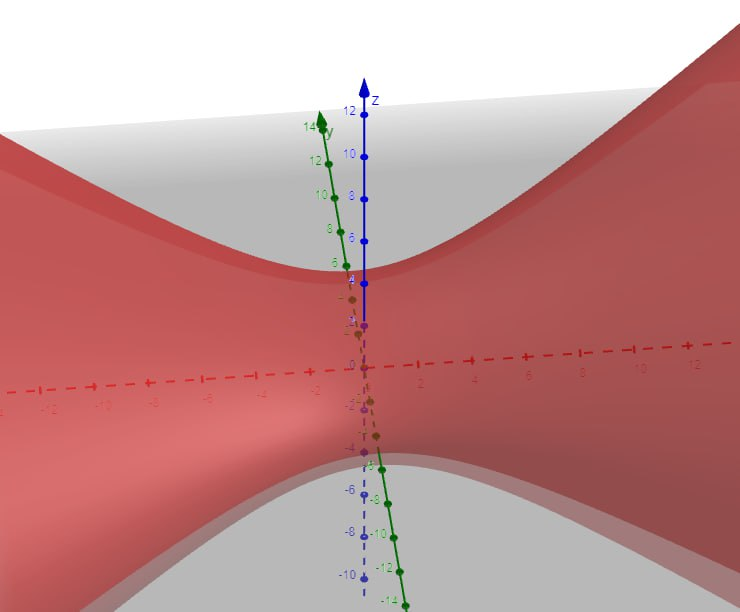
\includegraphics[height=200px]{rgr2.2.jpg} \\
    Первая картинка демонстрирует однополостный гиперболоид в исходном базисе а также новый базис, в котором уравнение однополостного гиперболоида принимает канонический вид. На второй картинке демонстрируется однополостный гиперболоид в новом базисе, в котором уравнение однополостного гиперболоида принимает канонический вид. Исходя из вида графиков мы можем сделать вывод, что в найденном базисе уравнение однополостного гиперболоида принимает канонический вид.
    

% task 3
\newpage
    \section{Линейный оператор и спектральный анализ}
    \subsection{Дано пространство геометрических векторов $\mathbb{R}$, его подпространства $L_1$ и $L_2$ и линейный оператор $\mathcal{A} : \mathbb{R}^3 \to \mathbb{R}^3$ }
    \subsubsection{Изобразите на графике подпространства $L_1$ и $L_2$.}
    Изобразим подпространства $L_1$ и $L_2$ на графике. Подпространства представляют собой плоскости в трехмерном пространстве $\mathbb{R}^3$  $L_1$ определяется системой уравнений: $x-y+z=0$ и $2x - 3y+4z=0$ и представляет собой пересечение 2 пересекающихся плоскостей в трехмерном пространстве $R_3$, то есть прямую. Найдем ее уравнение:\\
    \begin{equation*}
        \begin{cases}
            $x-y+z=0$ \\
            $2x-3y+4z=0$\\
        \end{cases}
        \begin{cases}
            $y = x+z$\\
            $2x-3x-3z+4z=0$\\
        \end{cases}
        \begin{cases}
            $y=x+z$\\
            $x=z$\\
        \end{cases}
        \begin{cases}
            $y=2z$\\
            $x=z$\\
        \end{cases}
    \end{equation*}
    пусть $z=t$, тогда $x = t$, $y = 2t$; \\
    Получили направляющий вектор прямой $L_1$ $(1, 2, 1)$, также прямая проходит через точку $(0, 0, 0)$\\
    Тогда уравнение прямой имеет вид:\\
    $\frac{x}{1}=\frac{y}{2}=\frac{z}{1}$\\
    $L_2$ задано уравнением $2x+3y-4z=0$. Оно представляет собой плоскость в трехмерном пространстве. \\
    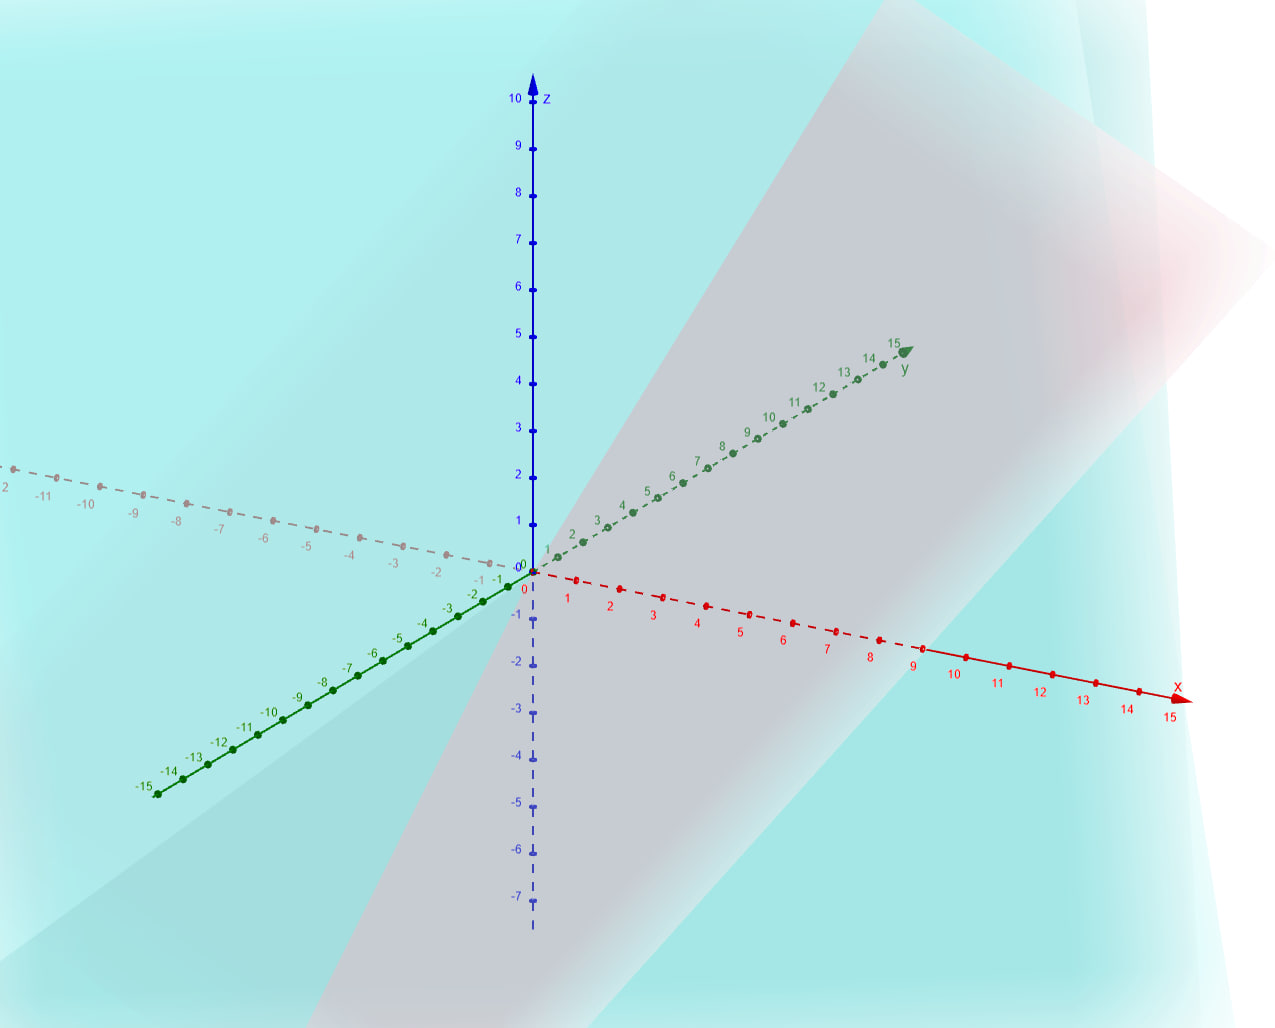
\includegraphics[height=200px]{rgr3.1.jpg}
    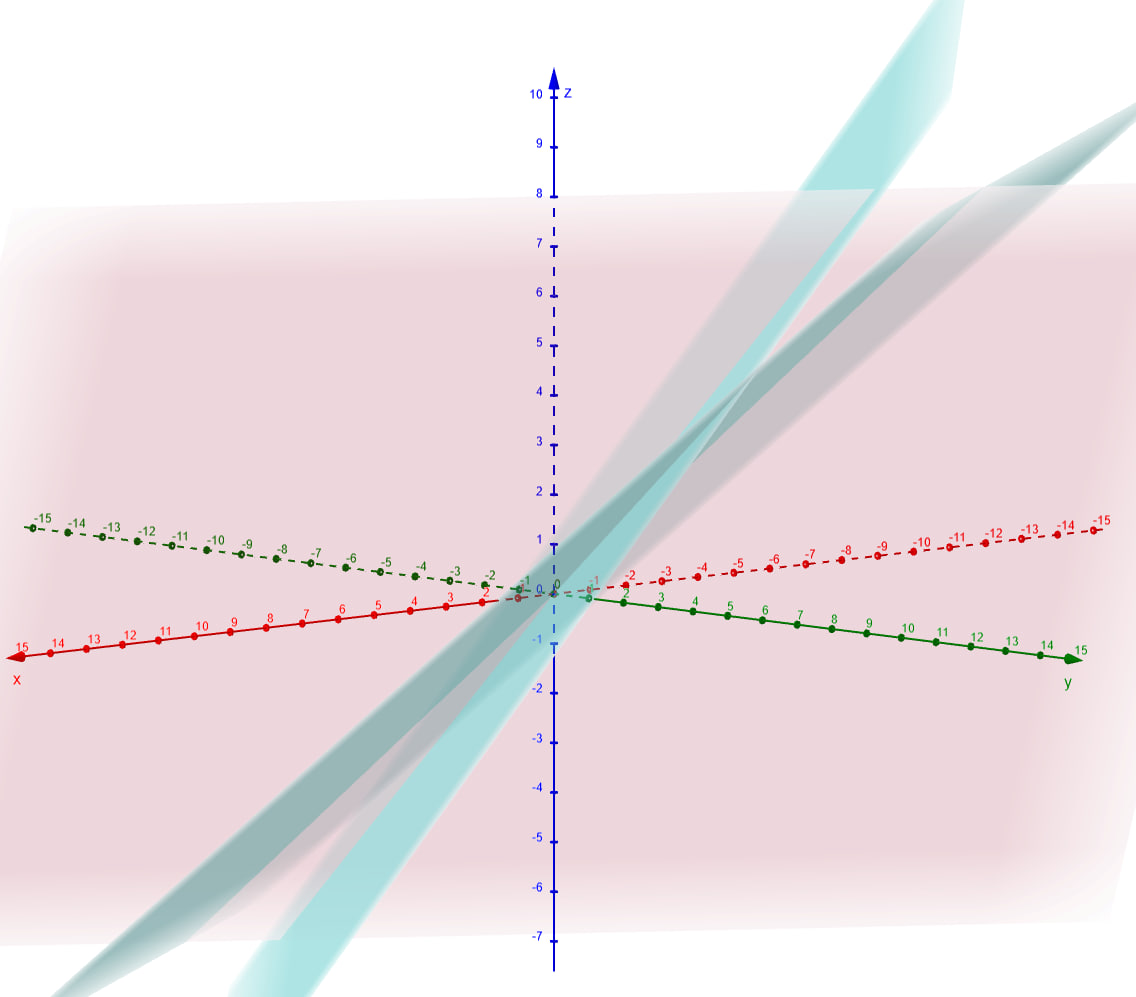
\includegraphics[height=200px]{rgr3.2.jpg}
    
    \subsubsection{Методами аналитической геометрии составьте формулу для линейного оператора $\mathcal{A}$.}
    Пусть $M_0 (x_0, y_0, z_0)$ - произвольная точка пространства $\mathbb{R}^3$.\\
    $L_3$ - подпространство, параллельное $L_2$, $L_3 \bigcap L_1 = M_1, M_1 (x_1, y_1, z_1)$.\\
    Составим формулу для линейного оператора A - оператора проектирования пространства $\mathbb{R}^3$ на подпространство $L_1$ параллельно $L_2$: $A(M_0) = M_1$ \\
    Уравнение плоскости $L_3 || L_2: 2(x-x_0) + 3(y-y_0) - 4(z-z_0) = 0$ \\
    $2x+3y-4z = 2x_0 + 3y_0 - 4z_0$ \\
    Получаем систему нахождения координат $M_1 ( x_1, y_1, z_1)$.\\
    \begin{equation*}
        \begin{cases}
            x - y + z = 0 \text{   (1)} \\
            2x - 3y + 4z = 0 \text{   (2)}\\
            2x-3y+4z = 2x_0 + 3y_0 - 4z_0 \text{   (3)}\\
        \end{cases}
    \end{equation*}
    Пусть $z=t$, тогда из (1) $x - y + t = 0 => x = y - t$\\
    Из (2): $2(y-t) - 3y + 4t = 0$ \\
    $2y - 2t - 3y + 4t = 0$ \\
    $-y + 2t = 0$ \\
    $y = 2t$\\
    Подставим $y = 2t$ в $x = y - t$  :  $x = 2t - t = t $\\
    Координаты точки $M_1$ имеют вид $(x_1, y_1, z_1) = (t,2t,t)$\\
    Теперь выразим $t$ через $x_0, y_0, z_0$ \\
    Подставим координаты $M_1$ в уравнение $2x + 3y - 4z = 2x_0 + 3y_0 - 4 z_0$ \\
    $2t + 3(2t) - 4t = 2x_0 + 3y_0 - 4z_0$ \\
    $2t + 6t - 4t = 2x_0 + 3y_0 - 4z_0$\\
    $4t = 2x_0 + 3y_0 - 4z_0$\\
    $t = \frac{2x_0 + 3y_0 - 4z_0}{4}$\\
    Тогда формула линейного оператора $A$ имеет вид:\\
    $A(M_0) = (x_1, y_1, z_1) = (\frac{2x_0 + 3y_0 - 4z_0}{4},2 \cdot \frac{2x_0 + 3y_0 - 4z_0}{4}, \frac{2x_0 + 3y_0 - 4z_0}{4})$ \\
    $A(x_0, y_0, z_0) =(\frac{2x_0 + 3y_0 - 4z_0}{4}, \frac{2x_0 + 3y_0 - 4z_0}{2}, \frac{2x_0 + 3y_0 - 4z_0}{4})$ \\
  
    \subsubsection{Составьте его матрицу в базисе $\{\overrightarrow{i}, \overrightarrow{j}, \overrightarrow{k}\}$ пространства $\mathbb{R}^3$}
    $A(\overrightarrow{i}) = A(1,0,0) = (\frac{2*1+3*0-4*0}{4}, \frac{2*1+3*0-4*0}{2}, \frac{2*1+3*0-4*0}{4}) = (\frac{2}{4}, \frac{2}{2}, \frac{2}{4}) = (\frac{1}{2}, 1, \frac{1}{2})$\\ 
    $A(\overrightarrow{j}) = A(0,1,0) = (\frac{2*0+3*1-4*0}{4}, \frac{2*0+3*1-4*0}{2}, \frac{2*0+3*1-4*0}{4}) = (\frac{3}{4}, \frac{3}{2}, \frac{3}{4})$\\ 
    $A(\overrightarrow{k}) = A(0,0,1) = (\frac{2*0+3*0-4*1}{4}, \frac{2*0+3*0-4*1}{2}, \frac{2*0+3*0-4*1}{4}) = ( - \frac{4}{4},- \frac{4}{2},- \frac{4}{4}) = (-1, -2, -1)$\\ 
    Матрица линейного оператора $A$ в базисе ${\overrightarrow{i}, \overrightarrow{j}, \overrightarrow{k}}$ имеет вид: \\
        \begin{equation*}
    A = 
        \begin{pmatrix}
            \frac{1}{2}& \frac{3}{4}& -1\\
            1& \frac{3}{2}& -2\\
            \frac{1}{2}& \frac{3}{4}& -1\\
        \end{pmatrix}
    \end{equation*}
    
    \subsubsection{Решите задачу о диагонализации полученной матрицы методом спектрального анализа.}
    Для начала найдем собственные числа оператора. Для этого решим
    уравнение $det(A - \lambda  \cdot  E)=0$
    \\
    \begin{equation*}
        \begin{vmatrix}
            \frac{1}{2} - \lambda & \frac{3}{4}& -1\\
            1& \frac{3}{2}-\lambda& -2\\
            \frac{1}{2}& \frac{3}{4}& -1-\lambda\\    
        \end{vmatrix}
        = 0
    \end{equation*}
    $(\frac{1}{2} - \lambda)(\frac{3}{2} - \lambda)(-1-\lambda) + \frac{3}{4}(-2)\frac{1}{2}+(-1)\cdot 1 \cdot \frac{3}{4} - (\frac{1}{2}(\frac{3}{2} - \lambda)(-1)+\frac{3}{4}(-2)(\frac{1}{2} -\lambda) +(-1-\lambda)\cdot 1 \cdot \frac{3}{4}) = 0$\\
    \\
    $(\frac{3}{4} - 2 \lambda + \lambda^2)(-1-\lambda) - \frac{3}{4} - \frac{3}{4} - (-\frac{3}{4} + \frac{1}{2}\lambda - \frac{3}{4} + \frac{3}{2}\lambda - \frac{3}{4} - \frac{3}{4}\lambda)=0$\\
    \\
    $-\frac{3}{4} - \frac{3}{4}\lambda + 2\lambda + 2\lambda^2 - \lambda^2-\lambda^3 - \frac{3}{4} -\frac{3}{4} - (-\frac{9}{4} + \frac{5}{4}\lambda) = 0$\\
    \\
    $\lambda^2 - \lambda^3 = 0$ \\
    \\
    $\lambda^2(1-\lambda) = 0$\\
    \\
    $\left[ 
      \begin{gathered} 
        \lambda^2 = 0 \\ 
        1 - \lambda = 0 \\ 
      \end{gathered} 
    \right.$
    $\left[ 
      \begin{gathered} 
        \lambda = 0 \\ 
        \lambda = 1 \\ 
      \end{gathered} 
    \right.$ \\
    Составим матрицу с полученными $\lambda_{1,2} = 0, \lambda_3 = 1$\\
    \begin{equation*}
        \begin{pmatrix}
            0& 0& 0\\
            0& 0& 0\\
            0& 0& 1\\
        \end{pmatrix}
    \end{equation*}
    Найдём собственные векторы.
    $\lambda_{1,2} = 0$
    \begin{equation*}
    A -\lambda E = 
        \begin{pmatrix}
            \frac{1}{2}& \frac{3}{4}& -1\\
            1& \frac{3}{2}& -2\\
            \frac{1}{2}& \frac{3}{4}& -1\\
        \end{pmatrix}
    \end{equation*}
    \begin{equation*}
        \begin{pmatrix}
            \frac{1}{2}& \frac{3}{4}& -1 \text{ |  0}\\
            1& \frac{3}{2}& -2 \text{ |  0}\\
            \frac{1}{2}& \frac{3}{4}& -1\text{ |  0}\\
        \end{pmatrix}
        \sim{~} 
        \begin{pmatrix}
            \frac{1}{2}& \frac{3}{4}& -1 \text{ |  0}\\
            1& \frac{3}{2}& -2 \text{ |  0}\\
            0& 0& 0\text{ |  0}\\
        \end{pmatrix}
        \sim{~} 
        \begin{pmatrix}
            \frac{1}{2}& \frac{3}{4}& -1 \text{ |  0}\\
            0& 0& 0 \text{ |  0}\\
            0& 0& 0\text{ |  0}\\
        \end{pmatrix}
    \end{equation*}
    Получим
    \begin{equation*}
        \begin{cases}
            \frac{1}{2}x_1 + \frac{3}{4}x_2 - x_3 = 0 \\
            x_3 = \frac{1}{2}x_1 + \frac{3}{4}x_2 \\
        \end{cases}
        =>
        \begin{cases}
            x_1 = a_1, a_1 \in \mathbb{R} \\
            x_2 = a_2, a_2 \in \mathbb{R} \\
            x_3 = \frac{1}{2}a_1 + \frac{3}{4}a_2
        \end{cases}
    \end{equation*}
    Пусть $a_1 = 1, a_2 = 0$, тогда $x_3 = \frac{1}{2}$. Получим собственный вектор $\overrightarrow{b_1}(1,0,\frac{1}{2})$ \\
    при $a_1 = 0, a_2 = 1$, получаем $x_3 = \frac{3}{4}$ и собственный вектор $\overrightarrow{b_2}(0,1,\frac{3}{4})$ \\
    2. $\lambda_3 = 1$ \\
    $A - \lambda E = 0$ \\
    \begin{equation*}
        A -\lambda E = 
        \begin{pmatrix}
            -\frac{1}{2}& \frac{3}{4}& -1\\
            1& \frac{1}{2}& -2\\
            \frac{1}{2}& \frac{3}{4}& -2\\
        \end{pmatrix}
    \end{equation*}
    \begin{equation*}
        \begin{pmatrix}
            -\frac{1}{2}& \frac{3}{4}& -1 \text{ |  0}\\
            1& \frac{1}{2}& -2 \text{ |  0}\\
            \frac{1}{2}& \frac{3}{4}& -2\text{ |  0}\\
        \end{pmatrix}
        \sim{~} 
        \begin{pmatrix}
            -\frac{1}{2}& \frac{3}{4}& -1 \text{ |  0}\\
            0& 2& -4 \text{ |  0}\\
            0& \frac{3}{2}& -3\text{ |  0}\\
        \end{pmatrix}
        \sim{~} 
        \begin{pmatrix}
            -\frac{1}{2}& \frac{3}{4}& -1 \text{ |  0}\\
            0& 2& -4 \text{ |  0}\\
            0& 0& 0\text{ |  0}\\
        \end{pmatrix}
    \end{equation*}
    Получим систему
    \begin{equation*}
        \begin{cases}
            -\frac{1}{2}x_1 + \frac{3}{4}x_2 - x_3 = 0 \\
            2x_2 - 4 x_3 = 0 \\
        \end{cases}
    \end{equation*}  
    \begin{equation*}
        \begin{cases}
            x_1 = \frac{3}{2}x_2 - 2 x_3\\
            x_2 = 2x_3
        \end{cases}
    \end{equation*}
    \begin{equation*}
        \begin{cases}
            x_1 = 3x_3 - 2x_3\\
            x_2 = 2x_3
        \end{cases}
    \end{equation*}
    \begin{equation*}
        \begin{cases}
            x_1 = x_3 \text{  Пусть, $x_3 = a, a \in \mathbbb{R}$, тогда $x_1 = a, x_2 = 2a$}\\
            x_2 = 2x_3 \text{  При $a = 1$ получим собственный вектор $\overrightarrow{b_3}(1,2,1)$}
        \end{cases}
    \end{equation*}
    Найдем базис, в котором матрица линейного оператора $A$ имеет диагональный вид. \\
    Пусть этот базис $E = \{ \overrightarrow{e_1},\overrightarrow{e_2},\overrightarrow{e_3} \}$ \\
    $\overrightarrow{e_1} = 1(1,0,0) + \frac{1}{2}(0,0,1) = (1,0,\frac{1}{2}) $ \\
    \\
    $\overrightarrow{e_2} = 1(0,1,0) + \frac{3}{4}(0,0,1) = (0,1,\frac{3}{4})  $ \\
    \\
    $\overrightarrow{e_3} = 1(1,0,0) + 2(0,1,0) +1(0,0,1) = (1,2,1)  $ \\
    \subsubsection{На построенном ранее графике изобразите базис, в котором матрица линейного оператора $\mathcal{A}$ имеет диагональный вид. Объясните его смысл.}
    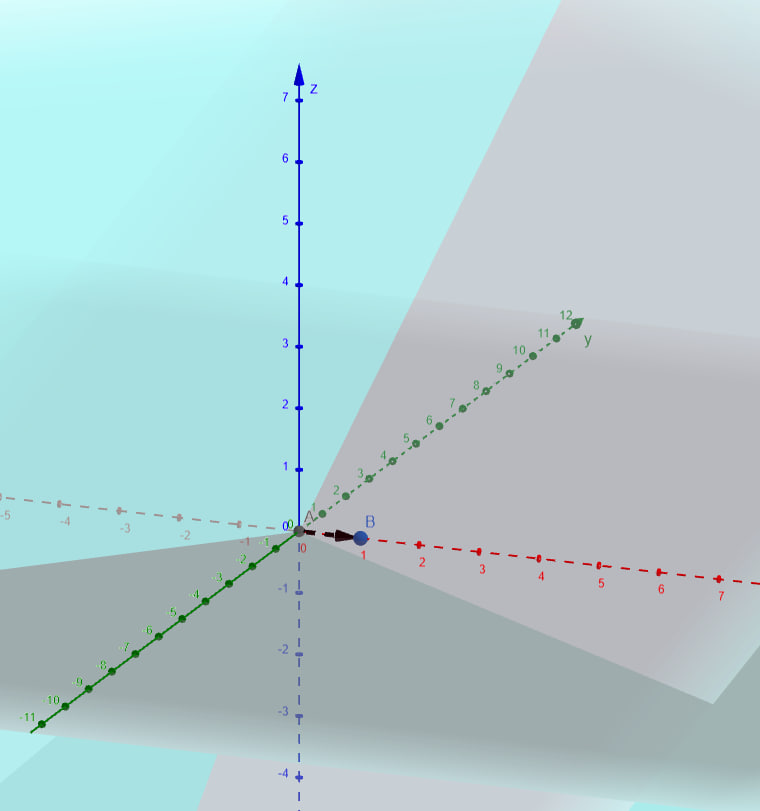
\includegraphics[height=200px]{rgr3.3.jpg}
    \\
    Базис в котором матрица оператора имеет диагональный вид, содержит на главной диагонали собственныe числа этого оператора и состоит из его собственных векторов.
    \subsection{Дано пространство функций $L$, отображение $\mathcal{A} L \to L$ и вектор $p(t) \in L$}
    
    \subsubsection{Выберите базис $L$ и докажите что это базис}
    Для того чтобы выбрать базис в пространстве многочленов степени не
    выше второй с вещественными коэффициентами, нужно найти три
    линейно независимых многочлена, которые образуют базис этого
    пространства.\\
    Давайте рассмотрим многочлены, которые представлены в данной
    задаче:\\
    $f_1(t) = 1$\\
    $f_2(t) = t$\\
    $f_3(t) = t^2$\\
    Проверим, являются ли такая система линейно независимой:\\
    Предположим, что существуют такие константы $c_1$, $c_2$, и $c_3$, хотя бы одна
    из которых не равна нулю, такие что:\\
    $c_1  \cdot  f_1(t) + c_2  \cdot  f_2(t) + c_3  \cdot  f_3(t)=0$\\
    тогда $c_1 + c_2  \cdot  t+c_3  \cdot  t^2 = 0$\\
    Это равенство должно выполняться для всех значений $t$. Рассмотрим
    несколько значений $t$:\\
    При $t = 0$: $c_1 = 0$\\
    При $t = 1$: $c_1 + c_2 + c_3 = 0$\\
    При $t =-1$: $c_1 - c_2 + c_3 = 0$\\
    Теперь решим эту систему уравнений:\\
    Из первого уравнения $c_1 = 0$, а затем, подставив $c_1 = 0$ во второе и третье
    уравнения, получаем $c_2 = c_3 = 0$.\\
    Таким образом, многочлены $f_1(t)=1$, $f_2(t)=t$ и $f_3(t)=t^2$ являются линейно
    независимыми.\\
    Таким образом, они образуют базис пространства многочленов степени
    не выше второй с вещественными коэффициентами.\\
    
    \subsubsection{Убедитесь, что отображение $\mathcal{A}$ является линейным (оператором).}
    Чтобы убедиться, что отображение A является линейным оператором,
    нужно проверить два условия: \\
    1. Аддитивность:\\
    Пусть f(t) и g(t) - произвольные многочлены степени не выше второй.\\
    Тогда:\\
    $A(f + g) = (f + g)'' - 3(f + g)' + (f + g) = f '' + g'' - 3f ' - 3g' + f + g = (f '' - 3f ' + f) + (g'' -
    3g' + g) = A(f) + A(g)$ - выполняется\\
    2. Гомогенность:\\
    Пусть f(t) - произвольный многочлен степени не выше второй, $a \in R$ -
    произвольное число. Тогда:\\
    $A(af) = (af)'' - 3(af)' + af = a \cdot  f '' - 3 \cdot  a  \cdot  f ' + a \cdot  f = a(f '' - 3f ' + f) = a \cdot  A(f)$ -
    выполняется\\
    Таким образом, отображение А является линейным оператором.\\
    
    \subsubsection{Найдите матрицу оператора $\mathcal{A}$ в выбранном базисе и его ранг.}
    Чтобы найти матрицу оператора $A$ в выбранном базисе, мы должны
    вычислить образы базисных векторов под действием оператора $A$ и
    представить эти образы в координатном виде относительно выбранного
    базиса. \\
    1. Образ многочлена 1 под действием $A$:\\
    $A(1) = 1'' - 3  \cdot  1' + 1 = 1$\\
    2. Образ многочлена t под действием $A$:\\
    $A(t) = t'' - 3  \cdot  t' + t = -3 + t$\\
    3. Образ многочлена $t^2$ под действием $A$:\\
    $A(t^2) = (t^2)'' - 3  \cdot  (t^2)' + t^2 = 2t‘ - 6t + t^2 = 2 - 6t + t^2$\\
    Теперь представим каждый из этих образов в виде линейной
    комбинации базисных элементов $1$, $t$ и $t^2$:\\
    1. Образ многочлена $1$:\\
    $0 = 1  \cdot  1 + 0  \cdot  t + 0  \cdot  t^2 \Rightarrow (1, 0, 0)$\\
    2. Образ многочлена $t$:\\
    $-3 + t = -3  \cdot  1 + 1  \cdot  t + 0  \cdot  t^2 \Rightarrow (-3, 1, 0)$\\
    3. Образ многочлена $t^2$:\\
    $2 - 6t + t^2 = 2  \cdot  1 - 6  \cdot  t + 1  \cdot  t^2 \Rightarrow (2, -6, 1)$\\
    Теперь мы можем записать эти коэффициенты в матрицу, где каждый
    столбец представляет координаты образа соответствующего базисного
    вектора в выбранном базисе:
    \\
    \begin{equation*}
        A =
        \begin{pmatrix}
            1& -3& 2\\
            0& 1& -6\\
            0& 0& 1\\
        \end{pmatrix}
    \end{equation*}
    \\
    Это и есть матрица оператора $A$ в выбранном базисе. \\
    Чтобы найти ранг матрицы, заметим что она уже имеет ступенчатый вид,
    посчитаем количество ненулевых строк. Их две, поэтому ранг матрицы
    оператора $A$ равен $2$. \\
    
    \subsubsection{Найдите размерности ядра и образа оператора $\mathcal{A}$}
    Чтобы найти размерность ядра, мы должны решить уравнение $Af=0$,
    то есть найти все многочлены $f(t)$, для которых $Af=0$.\\
    $f'' - 3f' + f = 0 \\
    f(t) = a  \cdot  t^2 + b \cdot  t + c$\\
    $(a  \cdot  t^2 + b \cdot  t + c)'' + (a  \cdot  t^2 + b \cdot  t + c)’ + a  \cdot  t^2 + b \cdot  t + c = 0$\\
    $(2a  \cdot  t + b)’ + 2a  \cdot  t + b + a  \cdot  t^2 + b \cdot  t + c = 0$\\
    $2a + 2a  \cdot  t + b + a  \cdot  t^2 + b \cdot  t + c = 0$\\
    $a  \cdot  t^2 + (2a + b) t + (2a + b + c) = 0$\\
    Получили систему:\\
    \begin{equation*}
            \begin{cases}
                a = 0 \\
                2a + b = 0 \\
                2a + b + c = 0 \\
            \end{cases}
            \Rightarrow
            \begin{cases}
                a = 0 \\
                b = 0 \\
                c = 0 \\
            \end{cases}
        \end{equation*}
    $Ker A = {0 \cdot  t^2 + 0 \cdot  t + 0} = {(0, 0, 0)}$\\
    Размерность $Ker \; A$ равна $1$.\\
    Теперь чтобы найти размерность образа $Im \; A$ воспользуемся теоремой
    о размерностях ядра и образа: \\
    Сумма размерностей ядра и образа любого линейного отображения\\
    $A: V \to W$ равна размерности пространства прообразов: \\
    $dim \; ker \; A + dim \; im \; A = dim \; V$ \\
    в нашем случае $dim \; Ker \; A = 1$, $dim \; L = 3$ (так как $L$ пространство
    многочленов не выше $2$ степени)\\
    Тогда $dim \; Im \; A = dim \; L - dim \; Ker \; A = 3 - 1 = 2$
    
    \subsubsection{Найдите собственные числа и векторы оператора. Определите размерность пространства собственных векторов и сделайте вывод о диагонализируемости матрицы оператора.}
    Прежде всего найдем собственные числа оператора. Для этого решим
    уравнение $det(A - \lambda E)=0$ \\
    \begin{equation*}
        \begin{vmatrix}
            1 - \lambda& -3& 2\\
            0& 1 - \lambda& -6\\
            0& 0& 1 - \lambda \\
        \end{vmatrix}
        = 0
    \end{equation*}
    \\
    $-\lambda^3 + 3  \cdot  \lambda^2 - 3\lambda+1 = 0$ \\
    $-(\lambda - 1)^3 = 0$\\
    $\lambda = 1$ - собственное число
    Найдем собственный вектор соответствующий $\lambda = 1$
    \\
    \begin{equation*}
        \begin{pmatrix}
            1-1& -3& 2\\
            0& 1-1& -6\\
            0& 0& 1-1\\    
        \end{pmatrix}
        \begin{pmatrix}
            $x_1$\\
            $x_2$\\
            $x_3$\\
        \end{pmatrix}
        =
        \begin{pmatrix}
            0\\
            0\\
            0\\
        \end{pmatrix}
    \end{equation*}
    \\
    \begin{equation*}
        \begin{pmatrix}
            0& -3& 2\\
            0& 0& -6\\
            0& 0& 0\\    
        \end{pmatrix}
        \begin{pmatrix}
            $x_1$\\
            $x_2$\\
            $x_3$\\
        \end{pmatrix}
        =
        \begin{pmatrix}
            0\\
            0\\
            0\\
        \end{pmatrix}
    \end{equation*}
    получили систему уравнений: \\
    \begin{equation*}
            \begin{cases}
                -3  \cdot  x_2 + 2  \cdot  x_3 = 0 \\
                -6  \cdot  x_3 = 0 \\
            \end{cases}
        \end{equation*}
    Откуда общее решение: $x_1 = a$, $x_2 = 0$, $x_3 = 0$ \\
    пусть $x_1 = 1$, тогда $v = (1, 0, 0)^T$ - собственный вектор \\
    Размерность пространства собственных векторов равна количеству
    линейно независимых собственных векторов. В данном случае, у нас
    есть только один собственный вектор, так как кратность собственного
    значения $\lambda = 1$ равна 3, но для этого собственного значения существует
    только один линейно независимый собственный вектор. Следовательно,
    размерность пространства собственных векторов равна 1. \\
    Матрицу оператора нельзя диагонализировать, поскольку у нас есть
    только один линейно независимый собственный вектор для данной
    матрицы, в то время как для диагонализации нужно три линейно
    независимых собственных вектора (так как $dim \; L = 3$). Поэтому данную
    матрицу нельзя диагонализовать. 
    
    \subsubsection{Найдите образ вектора $p(t)$ умножением на матрицу оператора. Проверьте результат дифференцированием.}
    Найдем образ вектора, соответствующего $p(t)$, с помощью умножения
    на матрицу оператора $A$: \\
    $p(t) = 3t^2 + t + 2 соответствует вектор (2, 1, 3)^T$ \\
    \begin{equation*}
        A * p(t) = 
        \begin{pmatrix}
            1& -3& 2\\
            0& 1& -6\\
            0& 0& 1\\
        \end{pmatrix}
        \begin{pmatrix}
            2\\
            1\\
            3\\
        \end{pmatrix}
        =
        \begin{pmatrix}
            5\\
            -17\\
            3\\
        \end{pmatrix}
    \end{equation*}
    $Ap(t) = (5, -17, 3) = 3* t^2 - 17 * t + 5$\\
    Проверим результат через дифференцирование: \\
$p(t) = 3t^2 + t + 2$ \\
$p’(t) = 6t + 1$ \\
$p(t)'' = 6$ \\
$Af = f'' - 3f′ + f = 6 - 3(6t + 1) + 3t^2 + t + 2 = 3t^2 -17t + 5 \Rightarrow (5, -17, 3)$\\
Таким образом матрица оператора была найдена верно.

    
% evaluation paper
\newpage
\[
\renewcommand{\arraystretch}{2}
\begin{tabular}{| c | c |}
 \hline
    \hugeУчастник & \hugeВклад в \% \\
 \hline
    \hugeКаренин Константин & \huge25 \\
 \hline
    \hugeГонин Сергей & \huge25 \\
 \hline
    \hugeТемиров Тимур & \huge25 \\
 \hline
    \hugeМалышева Алиса & \huge25 \\
 \hline
\end{tabular}
\]
\end{document}